\documentclass[11pt,a4paper]{article}
\usepackage[T1]{fontenc}
\usepackage[utf8]{inputenc}
\usepackage[polish]{babel}
\usepackage{lmodern}
\usepackage{textcomp}
\usepackage[a4paper,margin=2.5cm]{geometry}
\usepackage{graphicx}
\usepackage{booktabs}
\usepackage{amsmath}
\usepackage{xcolor}
\usepackage{listings}
\usepackage{caption}
\usepackage[colorlinks=true,linkcolor=blue!50!black,citecolor=blue!50!black,urlcolor=blue!50!black]{hyperref}
\usepackage{float}

\captionsetup{font=small,labelfont=bf}
\captionsetup[table]{position=above}
\captionsetup[figure]{position=below}

\definecolor{kwcol}{RGB}{40,60,130}
\definecolor{cmcol}{RGB}{90,120,90}
\definecolor{nrcol}{RGB}{130,130,130}
\definecolor{bgcol}{RGB}{248,248,248}
\lstdefinestyle{cpp}{
  language=C++,
  basicstyle=\ttfamily\scriptsize,
  keywordstyle=\color{kwcol},
  commentstyle=\color{cmcol}\itshape,
  numbers=none,
  backgroundcolor=\color{bgcol},
  frame=single,
  rulecolor=\color{nrcol!50},
  breaklines=true,
  showstringspaces=false,
  columns=fullflexible,
  keepspaces=true,
  literate={ą}{{\k{a}}}1 {ć}{{\'c}}1 {ę}{{\k{e}}}1 {ł}{{\l}}1 {ń}{{\'n}}1
           {ó}{{\'o}}1 {ś}{{\'s}}1 {ź}{{\'z}}1 {ż}{{\.z}}1,
}
\lstset{style=cpp}

% wygenerowane przez scripts/plots.py z results/raw.csv
\newcommand{\refFull}{5\,831}
\newcommand{\refQps}{171}
\newcommand{\refPdziewiecdziesiatpiec}{5\,823}
\newcommand{\ompSmax}{10,5}
\newcommand{\ompEmax}{0,65}
\newcommand{\ompSosiem}{7,6}
\newcommand{\ompJedenDoRef}{0,98}
\newcommand{\mpiSmax}{7,2}
\newcommand{\mpiEmax}{0,90}
\newcommand{\mpiSrdzenmax}{7,2}
\newcommand{\mpiKomunikacjamax}{1,1}
\newcommand{\mpiBazamax}{8,7}
\newcommand{\cudaFull}{77,90}
\newcommand{\cudaCore}{77,88}
\newcommand{\cudaBase}{7,7}
\newcommand{\cudaNoStreamFull}{77,97}
\newcommand{\cudaDoRef}{75}
\newcommand{\cublasFull}{13,73}
\newcommand{\cublasCore}{13,59}
\newcommand{\cublasBase}{8,2}
\newcommand{\cublasDoCuda}{5,7}
\newcommand{\cudaVram}{52}
\newcommand{\cublasVram}{434}
\newcommand{\cudaNajlepszyBlok}{256}
\newcommand{\cudaBlokKmax}{128}
\newcommand{\cudaGBsGlowny}{657}
\newcommand{\cudaQpsGlowny}{12\,837}
\newcommand{\cudaGBsNmax}{197}
\newcommand{\cudaQpsNmax}{384}
\newcommand{\cudaQpsQmin}{526}
\newcommand{\cudaQpsQmax}{12\,710}
\newcommand{\cublasQpsQmin}{1\,639}
\newcommand{\cublasQpsQmax}{72\,836}


\title{Projekt D03: wyszukiwanie wektorowe top-$k$\\\large wersja sekwencyjna, OpenMP, MPI i CUDA}
\author{Jakub Balicki}
\date{2026}

\begin{document}
\sloppy
\maketitle

\section{Problem, dane i metodologia}
Dla partii $Q$ zapytań i bazy $N$ wektorów wymiaru $D$ (\texttt{float32}) program zwraca dla każdego zapytania $k$ najbliższych wektorów bazy w~odległości euklidesowej: ich indeksy i~odległości, posortowane rosnąco. Przy równej odległości wygrywa mniejszy indeks, więc wynik jest jednoznaczny i~wszystkie wersje powinny zwracać ten sam ranking. We wszystkich wersjach porównywany jest kwadrat odległości, a~pierwiastek liczony jest tylko dla wyniku.

\paragraph{Dane.} Wektory bazy i zapytań losowane z rozkładu $\mathcal{N}(0,1)$ (\texttt{generate\_data.py}, ziarno 42). Każdy zestaw $(N, D)$ ma jeden plik z $10\,000$ zapytań; program czyta pierwsze $Q$ z nich, więc wszystkie wersje i wszystkie wielkości partii używają tych samych zapytań.

\paragraph{Konfiguracja.} Wszystkie parametry są w jednym pliku \texttt{experiments.conf}. Przypadek główny, wspólny dla wszystkich wersji: $N=10^5$, $D=128$, $Q=1000$, $k=10$. Osobno badam $N\in\{10^4,10^5,10^6\}$, $D\in\{32,\dots,512\}$, $k\in\{1,10,32,64\}$ i $Q\in\{1,\dots,10^4\}$, za każdym razem zmieniając jeden parametr przypadku głównego.

\paragraph{Pomiar.} Każda konfiguracja to 2~przebiegi rozgrzewkowe i~7~mierzonych powtórzeń, a każde powtórzenie to osobny wiersz w~\texttt{results/raw.csv}. W~tabelach podaję medianę i~rozstęp międzykwartylowy (IQR). Mierzone wielkości:
\begin{itemize}
\item \emph{czas pełny} partii -- obliczenia razem z komunikacją MPI (rozesłanie zapytań, zebranie wyników, scalanie) albo z kopiowaniem zapytań i~wyników między CPU i~GPU; z~niego liczę przepustowość $\mathrm{QPS}=Q/T_\text{pełny}$,
\item \emph{czas rdzenia} -- same obliczenia (MPI: najwolniejszy proces, CUDA: kernel),
\item jednorazowe przygotowanie bazy (podział \texttt{MPI\_Scatterv}, kopia na GPU) i wczytanie plików -- osobno, poza czasem partii,
\item \emph{P95} -- 95. percentyl opóźnienia zapytania obsługiwanego pojedynczo, ze 100 zapytań w~każdym powtórzeniu, w~każdej wersji tak samo (na GPU z~kopiami zapytania i~wyniku),
\item pamięć szczytowa: RSS procesu (MPI: suma procesów) i~pamięć zajęta na GPU.
\end{itemize}
Przyspieszenie $S(p)=T(1)/T(p)$ i efektywność $E(p)=S(p)/p$ liczę przy stałym problemie (przypadek główny). Pomiary MPI wykonałem na jednym komputerze, więc są \textbf{pomiarem lokalnym}: procesy dzielą rdzenie i~pamięć i~nie pokazują skalowalności klastra.

Sprzęt i oprogramowanie opisuje tabela~\ref{tab:env} (generowana z~\texttt{results/env.txt}).
\begin{table}[H]
\centering\footnotesize
\caption{Środowisko pomiarów.}\label{tab:env}
\begin{tabular}{@{}lp{10.5cm}@{}}
\toprule
data & 2026-11-16 21:37:26 \\
CPU & AMD Ryzen 7 5700X 8-Core Processor \\
rdzenie/wątki & 16 wątków sprzętowych \\
RAM & 32013 MiB \\
GPU & NVIDIA GeForce RTX 4060, 595.99.02, 8188 MiB \\
GPU przed pomiarami & wykorzystanie 0\%, 1214 MiB zajęte \\
obciążenie CPU (loadavg) & 0.93 0.41 0.25 \\
system & Linux 7.0.0-43-generic \\
g++ & g++ (Ubuntu 15.2.0-16ubuntu1) 15.2.0 \\
Open MPI & 5.0.10 \\
nvcc & Build cuda\_12.4.r12.4/compiler.34097967\_0 \\
python & Python 3.14.4, numpy 2.5.4 \\
rozgrzewka/powtórzenia/zapytania do P95 & 2/7/100 \\
w tle & kontenery innego projektu (partie-hadoop, partie-mongo) bez zadań; ich okresowe sprawdzenia stanu chwilowo zajmowały 1-3 wątki (zapis obciążenia co 60 s: 2 skoki mongosh ok. 120\% CPU o 22:04 i 22:07, w trakcie pomiarów D=512) \\
kontrola & D=512 (ref, OpenMP 16, MPI 8) powtórzone o 22:30 - mediana czasu ref +0.3\%, MPI +0.9\% względem tego pliku; w powtórce OpenMP trafił na skok obciążenia (java), więc w raw.csv zostaje pierwszy przebieg \\
\bottomrule
\end{tabular}

\end{table}

\section{Poprawność}
\texttt{tests/check.py} porównuje każdą wersję z~niezależną referencją w~\texttt{numpy} (\texttt{float64}) -- indeksy i~odległości z~tolerancją $10^{-4}$, dla kilku liczb wątków i~procesów. Przypadki brzegowe: $k=1$, $k=N$, $k>N$ (program odmawia), $N=1$, duplikaty i~wektory równe (remisy), wektor zerowy, kratka liczb całkowitych (wiele remisów), $N$ niepodzielne przez $p$, $D=1$ i~$D=517$ (nie wielokrotność 4). Wszystkie wersje przechodzą wszystkie przypadki. Wyjątek dotyczy tolerancji cuBLAS: wzór $\|q\|^2+\|b\|^2-2q\cdot b$ dla prawie identycznych wektorów odejmuje duże, prawie równe liczby, więc dla odległości bliskiej zera błąd sięga $10^{-3}$; dla tej wersji tolerancja wynosi $2\cdot10^{-3}$. Tabela~\ref{tab:ranking} porównuje rankingi przypadku głównego z~referencją.

\begin{table}[H]
\centering\small
\caption{Zgodność rankingów z~referencją, przypadek główny (1000 zapytań, $k=10$).}\label{tab:ranking}
\begin{tabular}{lrrr}
\toprule
Wersja & Zapytania identyczne z ref. & Różne pozycje & Maks. różnica odległości \\
\midrule
cuBLAS & 1000 / 1000 & 0 & $8\cdot 10^{-6}$ \\
CUDA & 1000 / 1000 & 0 & $5\cdot 10^{-6}$ \\
MPI, 8 procesów & 1000 / 1000 & 0 & $0$ \\
MPI+OpenMP, 4×4 & 1000 / 1000 & 0 & $0$ \\
OpenMP, 16 wątków & 1000 / 1000 & 0 & $0$ \\
\bottomrule
\end{tabular}

\end{table}

\section{Wersje programu}
\paragraph{Referencja} (\texttt{reference/topk\_ref.cpp}). Dla każdego zapytania liczy kwadraty odległości do wszystkich $N$ wektorów i~wybiera $k$ najmniejszych par (odległość, indeks) przez \texttt{std::partial\_sort}. Para porównuje się leksykograficznie, co od razu daje regułę remisów.

\paragraph{OpenMP} (\texttt{openmp/topk\_omp.cpp}). Przy partii zapytań wątki dzielą się zapytaniami (\texttt{schedule(dynamic, 1)}); każdy wątek liczy całe zapytanie i~ma własny kopiec $k$ najlepszych kandydatów, więc nie ma sekcji krytycznych ani operacji atomowych. Gdy zapytań jest mniej niż wątków (także przy pomiarze P95), wątki dzielą się bazą (\texttt{schedule(static)}), każdy ma lokalny kopiec, a~na końcu wątek główny scala $p\cdot k$ kandydatów.

\paragraph{MPI} (\texttt{mpi/topk\_mpi.cpp}). Proces 0 wczytuje dane, a \texttt{MPI\_Scatterv} raz dzieli bazę: proces $r$ dostaje $\lfloor N/p\rfloor$ wektorów, a pierwsze $N \bmod p$ procesów o~jeden więcej. Dla partii: \texttt{MPI\_Bcast} zapytań, lokalne top-$k$ na swojej części bazy (z~globalnymi indeksami), \texttt{MPI\_Gather} lokalnych wyników do procesu 0 i~scalenie $p\cdot k$ kandydatów na zapytanie. Przesyłane jest $Q\cdot k$ par od procesu, a~nie macierz odległości. Wariant hybrydowy (\texttt{-fopenmp}) dzieli zapytania partii między wątki procesu.

\paragraph{CUDA} (\texttt{cuda/topk\_cuda.cu}). Jeden blok obsługuje jedno zapytanie: wektor zapytania trafia do pamięci współdzielonej, wątek $t$ przegląda wektory bazy $t, t+T, t+2T,\dots$ (odczyt po \texttt{float4}) i~trzyma posortowaną listę $k$ najlepszych. Listy wątków są potem scalane drzewiasto w~$\log_2 T$ krokach (w kroku $s$ wątek $t<s$ scala swoją listę z~listą $t+s$). Baza jest kopiowana na GPU raz; partia jest dzielona na 4~strumienie, żeby kopie jednej części nakładały się na obliczenia innej. Pamięć współdzielona bloku to $T\cdot k\cdot 8 + 4D$ bajtów, a~RTX 4060 pozwala na 99~KiB, dlatego $k\le 64$, a~dla $k=64$ program zmniejsza blok do \cudaBlokKmax{} wątków.

\paragraph{cuBLAS} (\texttt{cuda/topk\_cublas.cu}), dodatkowa referencja wydajności. Biblioteka liczy tylko iloczyny $q\cdot b$ jednym mnożeniem macierzy (\texttt{cublasSgemm}); normy, złożenie odległości i~wybór top-$k$ (ten sam schemat co wyżej) to moje kernele. Macierz odległości ma $Q\times N$ elementów, więc partia jest liczona kawałkami zajmującymi najwyżej 512~MiB.

\section{Porównanie wersji w przypadku głównym}
\begin{table}[H]
\centering\small
\caption{Przypadek główny $N=10^5$, $D=128$, $Q=1000$, $k=10$. Mediana z 7 powtórzeń [IQR]; ostatnia kolumna to przyspieszenie względem referencji liczone z~czasu pełnego.}\label{tab:glowny}
\resizebox{\textwidth}{!}{\begin{tabular}{llrrrrrrr}
\toprule
Wersja & Konfiguracja & $T_\text{pełny}$ [ms] [IQR] & $T_\text{rdzeń}$ [ms] & QPS & P95 [\textmu s] & RAM [MiB] & VRAM [MiB] & $T_\text{ref}/T$ \\
\midrule
referencja & 1 wątek & 5\,831,2 [27,9] & 5\,831,2 & 171 & 5\,823 & 54 & -- & 1,0 \\
OpenMP & 16 wątków & 569,0 [0,9] & 569,0 & 1\,758 & 830 & 54 & -- & 10,2 \\
MPI & 8 procesów & 824,2 [1,3] & 823,1 & 1\,213 & 855 & 262 & -- & 7,1 \\
CUDA & blok 256 & 77,9 [0,1] & 77,9 & 12\,837 & 1\,941 & 226 & 52 & 74,9 \\
CUDA bez strumieni & blok 256 & 78,0 [0,1] & 77,9 & 12\,825 & 1\,945 & 226 & 52 & 74,8 \\
cuBLAS & SGEMM + selekcja & 13,7 [0,0] & 13,6 & 72\,819 & 613 & 410 & 434 & 424,6 \\
\bottomrule
\end{tabular}
}
\end{table}
Najwyższą przepustowość ma cuBLAS. Własny kernel CUDA jest \cudaDoRef{} razy szybszy od referencji, ale \cublasDoCuda{} razy wolniejszy od cuBLAS. Na procesorze OpenMP z~16 wątkami wyprzedza MPI z~8 procesami: korzysta z~16 wątków sprzętowych (8~rdzeni z~SMT), a MPI w~tej konfiguracji ma jeden proces na rdzeń. Rozrzut (IQR) jest mały w~porównaniu z~medianą.

Opóźnienie pojedynczego zapytania (P95) układa się inaczej niż przepustowość. Referencja potrzebuje \pRef{}~\textmu s. OpenMP (\pOmp{}~\textmu s) i~MPI (\pMpi{}~\textmu s) dzielą jedno zapytanie na wszystkie wątki lub procesy. Najkrótsze opóźnienie ma cuBLAS (\pCublas{}~\textmu s). Własny kernel CUDA (\pCuda{}~\textmu s) jest tu wolniejszy od CPU, bo jedno zapytanie to jeden blok, czyli tylko jeden multiprocesor GPU; kernel jest zaprojektowany pod przepustowość dużych partii, nie pod pojedyncze zapytania.

Wersje GPU zajmują więcej RAM-u niż wersje CPU, bo samo środowisko CUDA i~przypięta pamięć hosta zajmują stałą ilość pamięci, widoczną już dla najmniejszej bazy (rys.~\ref{fig:pamiec}, $N=10^4$). MPI sumuje RSS ośmiu procesów, z~których każdy ma kopię zapytań i~bufory wyników.

\section{OpenMP}
\begin{table}[H]
\centering\small
\caption{OpenMP, przypadek główny. $S(p)$ i $E(p)$ względem wersji OpenMP na 1~wątku.}\label{tab:omp}
\begin{tabular}{rrrrrr}
\toprule
Wątki $p$ & $T(p)$ [ms] [IQR] & $S(p)$ & $E(p)$ & $T_\text{ref}/T(p)$ & P95 [\textmu s] \\
\midrule
1 & 5\,947,2 [19,9] & 1,00 & 1,00 & 0,98 & 5\,898 \\
2 & 2\,971,7 [15,6] & 2,00 & 1,00 & 1,96 & 2\,977 \\
4 & 1\,491,1 [25,3] & 3,99 & 1,00 & 3,91 & 1\,526 \\
8 & 785,9 [7,9] & 7,57 & 0,95 & 7,42 & 864 \\
16 & 569,0 [0,9] & 10,45 & 0,65 & 10,25 & 830 \\
\bottomrule
\end{tabular}

\end{table}
\begin{figure}[H]
\centering
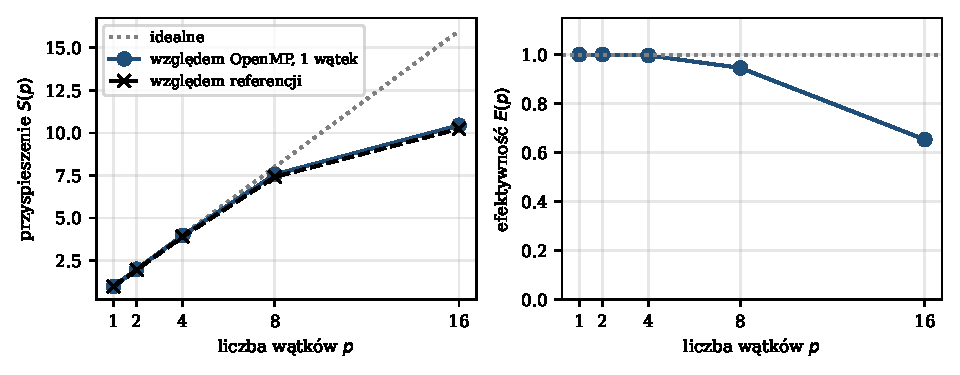
\includegraphics[width=0.9\textwidth]{fig/fig_omp.pdf}
\caption{OpenMP: przyspieszenie i efektywność, przypadek główny.}\label{fig:omp}
\end{figure}
Do 8~wątków przyspieszenie jest prawie liniowe ($S(8)=\ompSosiem$). Wątki nie współdzielą danych do zapisu, a~każdy ma własny kopiec, więc nic ich nie synchronizuje poza końcem pętli. Przy 16~wątkach $S=\ompSmax$, a~efektywność spada do \ompEmax: procesor ma 8~rdzeni, a~drugi wątek SMT na rdzeniu dzieli z~pierwszym jednostki wykonawcze, więc daje znacznie mniej niż dodatkowy rdzeń. Wersja OpenMP na jednym wątku ma praktycznie ten sam czas co referencja ($T_\text{ref}/T(1)=\ompJedenDoRef$), więc przyspieszenie względem referencji jest prawie takie samo jak $S(p)$.

\section{MPI}
\begin{table}[H]
\centering\small
\caption{MPI, przypadek główny, pomiar lokalny. Komunikacja = czas pełny $-$ czas rdzenia (Bcast, Gather, scalanie). $S$ i $E$ z~czasu pełnego względem $p=1$; dla wariantu hybrydowego $E$ liczona dla $p\cdot t$.}\label{tab:mpi}
\resizebox{\textwidth}{!}{\begin{tabular}{rrrrrrrrr}
\toprule
Procesy & Wątki & $T_\text{rdzeń}$ [ms] & Komunikacja [ms] & $T_\text{pełny}$ [ms] [IQR] & $S(p)$ & $E(p)$ & Scatterv bazy [ms] & RAM [MiB] \\
\midrule
1 & 1 & 5\,916,5 & 0,1 & 5\,916,6 [20,9] & 1,00 & 1,00 & 4,0 & 119 \\
2 & 1 & 2\,968,2 & 0,4 & 2\,968,6 [8,6] & 1,99 & 1,00 & 5,6 & 139 \\
4 & 1 & 1\,505,2 & 0,6 & 1\,505,8 [6,5] & 3,93 & 0,98 & 7,8 & 180 \\
8 & 1 & 823,1 & 1,1 & 824,2 [1,3] & 7,18 & 0,90 & 8,7 & 262 \\
8 & 2 & 842,4 & 1,1 & 843,5 [62,0] & 7,01 & 0,44 & 8,3 & 263 \\
4 & 4 & 596,6 & 0,8 & 597,4 [16,2] & 9,90 & 0,62 & 7,6 & 182 \\
2 & 8 & 583,4 & 0,5 & 583,8 [76,0] & 10,13 & 0,63 & 6,6 & 144 \\
\bottomrule
\end{tabular}
}
\end{table}
\begin{figure}[H]
\centering
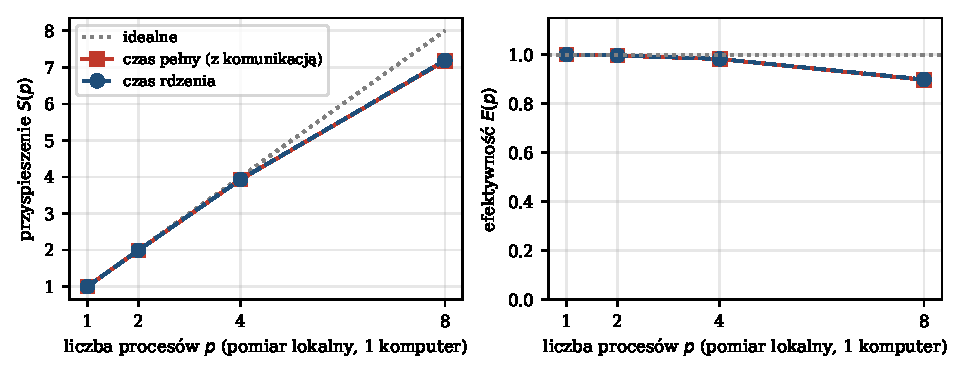
\includegraphics[width=0.9\textwidth]{fig/fig_mpi.pdf}
\caption{MPI: przyspieszenie i efektywność z czasu pełnego i czasu rdzenia (pomiar lokalny). Krzywe prawie się pokrywają, bo komunikacja trwa \mpiKomunikacjamax~ms.}\label{fig:mpi}
\end{figure}
MPI skaluje się podobnie do OpenMP do 8~procesów: $S(8)=\mpiSmax$, $E(8)=\mpiEmax$. Komunikacja na partię trwa tylko \mpiKomunikacjamax~ms, bo przesyłane są zapytania i~po $Q\cdot k$ par od procesu, a~nie odległości. Dlatego krzywe dla czasu pełnego i~czasu rdzenia na rys.~\ref{fig:mpi} prawie się pokrywają. Jednorazowe rozesłanie bazy (\mpiBazamax~ms dla 8~procesów) jest niewielkie wobec czasu partii. Spadek efektywności przy 8~procesach wynika z~tego, że procesy dzielą przepustowość pamięci i~pamięć podręczną L3 jednego procesora; to pomiar lokalny i~nie mówi nic o~skalowaniu na kilku komputerach. Wariant hybrydowy najlepiej wypada w~układzie $\hybrydaNajlepsza$ ($S=\hybrydaSmax$), czyli tak jak OpenMP na 16~wątkach -- znowu zysk z~wątków SMT.

\section{CUDA i cuBLAS}
\begin{table}[H]
\centering\small
\caption{CUDA: wpływ liczby wątków w bloku, przypadek główny.}\label{tab:bloki}
\begin{tabular}{rrrrr}
\toprule
Wątki w bloku & $T_\text{rdzeń}$ [ms] & $T_\text{pełny}$ [ms] & QPS & P95 [\textmu s] \\
\midrule
64 & 90,14 & 90,34 & 11\,069 & 5\,608 \\
128 & 82,57 & 82,06 & 12\,187 & 3\,192 \\
256 & 77,88 & 77,90 & 12\,837 & 1\,941 \\
512 & 79,33 & 79,37 & 12\,599 & 1\,741 \\
\bottomrule
\end{tabular}

\end{table}
\begin{figure}[H]
\centering
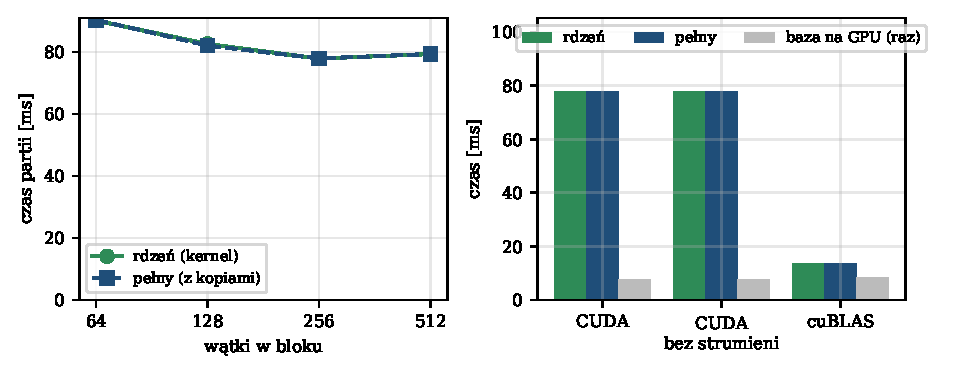
\includegraphics[width=0.9\textwidth]{fig/fig_cuda.pdf}
\caption{Lewo: czas partii w~zależności od liczby wątków w bloku. Prawo: czas rdzenia, pełny i jednorazowej kopii bazy dla własnego kernela (ze strumieniami i~bez) oraz cuBLAS.}\label{fig:cuda}
\end{figure}
Najlepszy czas daje blok \cudaNajlepszyBlok{} wątków. Przy 64~wątkach blok jest za mały, żeby zasłonić opóźnienia pamięci, a~przy 512 dłuższe jest scalanie list top-$k$ ($\log_2 T$ kroków) i~mniej bloków mieści się naraz na multiprocesorze. P95 maleje z~rozmiarem bloku, bo pojedyncze zapytanie liczy jeden blok -- im więcej w~nim wątków, tym szybciej. Strumienie nie dają mierzalnego zysku (\cudaFull~ms ze strumieniami i~\cudaNoStreamFull~ms bez): kopia 1000 zapytań to $Q\cdot D\cdot 4\approx 0{,}5$~MB i~trwa ułamek milisekundy, a~kernel kilkadziesiąt milisekund, więc nie ma czego nakładać. Z~tego samego powodu czas pełny jest praktycznie równy czasowi rdzenia. Czas rdzenia mierzony jest osobnym uruchomieniem kernela, więc w~pojedynczych przypadkach (np. $D=512$) wychodzi minimalnie większy od pełnego.

Kernel czyta całą bazę osobno dla każdego zapytania, czyli $Q\cdot N\cdot D\cdot 4$ bajty na partię. Dla przypadku głównego daje to \cudaGBsGlowny~GB/s, więcej niż przepustowość pamięci RTX 4060 (272~GB/s według producenta). Najpewniej bloki działające jednocześnie czytają w~przybliżeniu te same fragmenty bazy, więc część odczytów obsługuje pamięć podręczna L2. Wersja cuBLAS jest szybsza, bo mnożenie macierzy wykorzystuje każdy wektor bazy dla wielu zapytań naraz (kafelkowanie w~pamięci współdzielonej i~rejestrach). Płaci za to pamięcią: \cublasVram~MiB na GPU wobec \cudaVram~MiB własnego kernela.

\section{Wpływ $N$, $D$, $k$ i $Q$}
\begin{figure}[H]
\centering
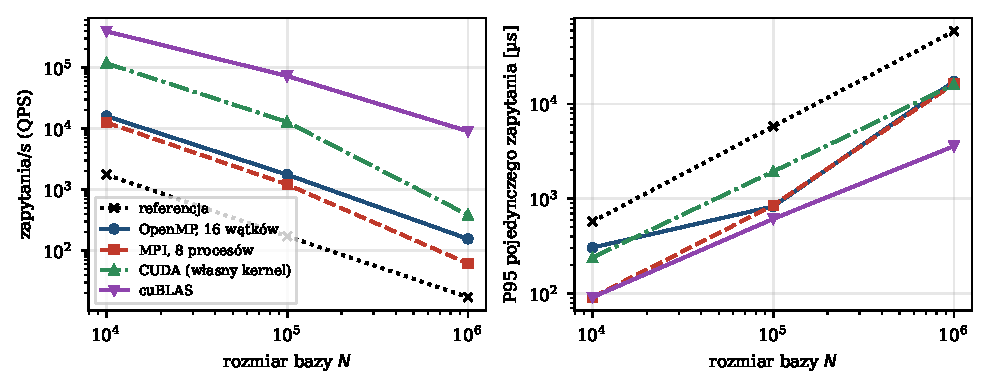
\includegraphics[width=0.9\textwidth]{fig/fig_n.pdf}
\caption{Przepustowość i P95 w zależności od $N$ ($D=128$, $Q=1000$, $k=10$).}\label{fig:n}
\end{figure}
\begin{figure}[H]
\centering
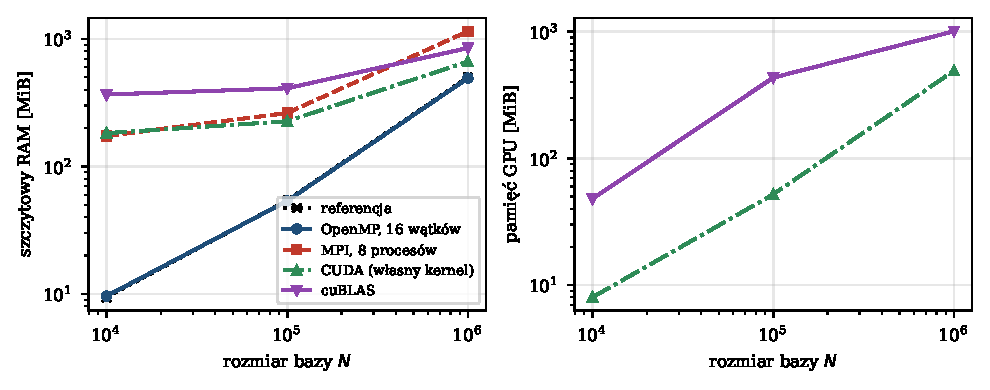
\includegraphics[width=0.9\textwidth]{fig/fig_pamiec.pdf}
\caption{Pamięć szczytowa w zależności od $N$: RAM (MPI -- suma procesów) i~pamięć GPU.}\label{fig:pamiec}
\end{figure}
\begin{figure}[H]
\centering
\begin{minipage}{0.48\textwidth}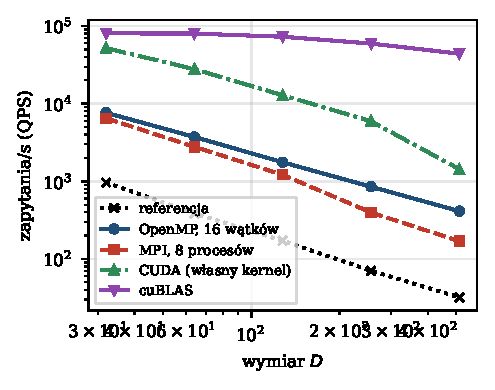
\includegraphics[width=\textwidth]{fig/fig_d.pdf}\end{minipage}\hfill
\begin{minipage}{0.48\textwidth}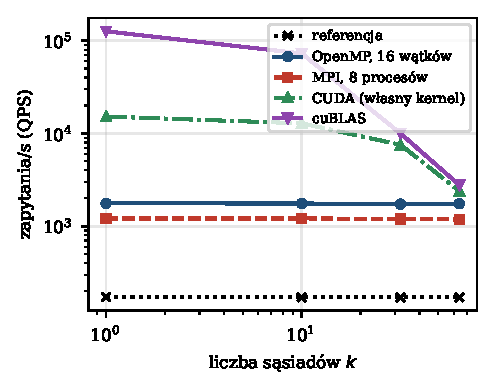
\includegraphics[width=\textwidth]{fig/fig_k.pdf}\end{minipage}
\caption{Przepustowość w zależności od $D$ (lewo) i $k$ (prawo).}\label{fig:dk}
\end{figure}
\begin{figure}[H]
\centering
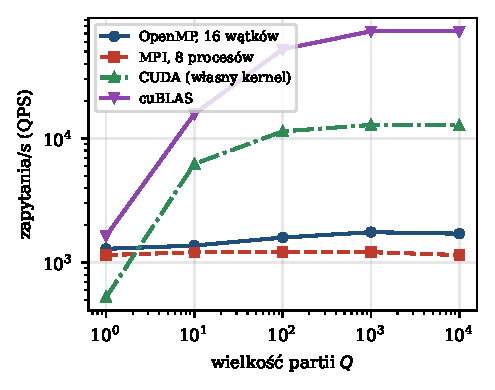
\includegraphics[width=0.5\textwidth]{fig/fig_q.pdf}
\caption{Przepustowość w zależności od wielkości partii $Q$ (bez referencji -- liczy zapytania po kolei, więc jej QPS nie zależy od $Q$).}\label{fig:q}
\end{figure}
\begin{table}[H]
\centering\small
\caption{Przepustowość (QPS, mediana) w zależności od $N$ (lewo) i $D$ (prawo); pozostałe parametry jak w przypadku głównym.}\label{tab:n}
\resizebox{0.49\textwidth}{!}{\begin{tabular}{rrrrrr}
\toprule
$N$ & referencja & OpenMP, 16 wątków & MPI, 8 procesów & CUDA (własny kernel) & cuBLAS \\
\midrule
10\,000 & 1\,752 & 16\,003 & 12\,620 & 117\,718 & 394\,462 \\
100\,000 & 171 & 1\,758 & 1\,213 & 12\,837 & 72\,819 \\
1\,000\,000 & 17 & 156 & 61 & 384 & 9\,052 \\
\bottomrule
\end{tabular}
}\hfill
\resizebox{0.49\textwidth}{!}{\begin{tabular}{rrrrrr}
\toprule
$D$ & referencja & OpenMP, 16 wątków & MPI, 8 procesów & CUDA (własny kernel) & cuBLAS \\
\midrule
32 & 964 & 7\,641 & 6\,492 & 51\,915 & 80\,513 \\
64 & 387 & 3\,725 & 2\,778 & 27\,821 & 80\,005 \\
128 & 171 & 1\,758 & 1\,213 & 12\,837 & 72\,819 \\
256 & 71 & 851 & 396 & 5\,935 & 59\,504 \\
512 & 32 & 413 & 169 & 1\,433 & 44\,058 \\
\bottomrule
\end{tabular}
}
\end{table}
\begin{table}[H]
\centering\small
\caption{Przepustowość (QPS, mediana) w zależności od $k$ (lewo) i wielkości partii $Q$ (prawo).}\label{tab:kq}
\resizebox{0.49\textwidth}{!}{\begin{tabular}{rrrrrr}
\toprule
$k$ & referencja & OpenMP, 16 wątków & MPI, 8 procesów & CUDA (własny kernel) & cuBLAS \\
\midrule
1 & 172 & 1\,762 & 1\,211 & 15\,213 & 126\,226 \\
10 & 171 & 1\,758 & 1\,213 & 12\,837 & 72\,819 \\
32 & 171 & 1\,730 & 1\,200 & 7\,539 & 10\,005 \\
64 & 171 & 1\,746 & 1\,180 & 2\,394 & 2\,774 \\
\bottomrule
\end{tabular}
}\hfill
\resizebox{0.42\textwidth}{!}{\begin{tabular}{rrrrr}
\toprule
$Q$ & OpenMP, 16 wątków & MPI, 8 procesów & CUDA (własny kernel) & cuBLAS \\
\midrule
1 & 1\,290 & 1\,149 & 526 & 1\,639 \\
10 & 1\,372 & 1\,212 & 6\,224 & 15\,770 \\
100 & 1\,591 & 1\,214 & 11\,391 & 52\,252 \\
1\,000 & 1\,758 & 1\,213 & 12\,837 & 72\,819 \\
10\,000 & 1\,709 & 1\,150 & 12\,710 & 72\,836 \\
\bottomrule
\end{tabular}
}
\end{table}

\paragraph{$N$.} Na CPU przepustowość maleje mniej więcej proporcjonalnie do $N$ (tab.~\ref{tab:n}). Własny kernel CUDA traci przy $N=10^6$ znacznie więcej (z~\cudaQpsGlowny{} do \cudaQpsNmax~QPS): baza ma 512~MB i~odczyty spadają do \cudaGBsNmax~GB/s, czyli blisko granicy pamięci karty. MPI przy $N=10^6$ odstaje od OpenMP. Przez procesor przechodzi wtedy odpowiednio \mpiGBsNmax{} i~\ompGBsNmax~GB/s danych bazy. Moje wyjaśnienie: w~OpenMP wątki liczą różne zapytania na tej samej bazie i~mogą korzystać z~tych samych linii w~pamięci podręcznej, a~procesy MPI czytają rozłączne części bazy, więc każdy bajt idzie z~pamięci RAM. P95 rośnie z~$N$ we wszystkich wersjach, a~zużycie pamięci rośnie liniowo z~rozmiarem bazy (rys.~\ref{fig:pamiec}).

\paragraph{$D$.} Koszt odległości rośnie liniowo z~$D$, więc przepustowość CPU spada z~$D$ (referencja: \refQpsDmin{} QPS dla $D=32$, \refQpsDmax{} dla $D=512$). cuBLAS prawie nie zależy od $D$ (\cublasQpsDmin{} i~\cublasQpsDmax~QPS), bo przy tej wielkości SGEMM jest szybkie, a~czas zajmuje głównie wybór top-$k$ z~macierzy odległości o~rozmiarze niezależnym od $D$.

\paragraph{$k$.} Na CPU $k$ nie ma znaczenia (OpenMP: \ompQpsKmin{} QPS dla $k=1$ i~\ompQpsKmax{} dla $k=64$), bo prawie każdy kandydat jest odrzucany jednym porównaniem ze szczytem kopca. Na GPU $k$ jest kluczowe: własny kernel spada z~\cudaQpsKmin{} do \cudaQpsKmax~QPS, a~cuBLAS z~\cublasQpsKmin{} do \cublasQpsKmax. Lista $k$ najlepszych w~każdym wątku to tablica w~pamięci lokalnej, wstawianie i~scalanie kosztują $O(k)$, a~dla $k=64$ blok musi być zmniejszony do \cudaBlokKmax{} wątków.

\paragraph{$Q$.} Na CPU przepustowość prawie nie zależy od wielkości partii; OpenMP przy $Q=1$ dzieli bazę między wątki i~osiąga \ompQpsQjeden{} QPS. Na GPU mała partia nie wypełnia karty: przy $Q=1$ działa jeden blok, a~do tego dochodzą kopie i~uruchomienie kernela, więc własny kernel ma \cudaQpsQmin{} QPS, a~dopiero od $Q\approx100$ zbliża się do maksimum (\cudaQpsQmax{} QPS dla $Q=10^4$).

\section{Wnioski}
\begin{itemize}
\item Wszystkie wersje zwracają ranking identyczny z~referencją dla 1000 zapytań przypadku głównego; różnice odległości są rzędu $10^{-6}$ na GPU.
\item OpenMP i~MPI skalują się prawie liniowo do liczby rdzeni (8). Wątki SMT dają dodatkowy, ale mniejszy zysk ($S=\ompSmax$ dla 16~wątków). Komunikacja MPI jest pomijalna, bo przesyłane są tylko lokalne top-$k$, a~nie odległości. Wszystkie pomiary MPI są lokalne.
\item GPU daje największą przepustowość dla dużych partii: własny kernel \cudaDoRef{}$\times$ szybciej od referencji, cuBLAS kolejne \cublasDoCuda{}$\times$ szybciej, kosztem pamięci GPU.
\item Własny kernel jest ograniczony przepustowością pamięci (przy $N=10^6$ czyta bazę z~prędkością bliską możliwościom karty) i~kosztem utrzymania listy top-$k$, który rośnie z~$k$. Dla pojedynczych zapytań i~małych partii wykorzystuje tylko część GPU i~ma większe opóźnienie niż OpenMP.
\item Ograniczenia: $k\le 64$ na GPU (pamięć współdzielona), pomiar MPI tylko na jednym komputerze, a~cuBLAS mniej dokładnie wyznacza bardzo małe odległości.
\end{itemize}

\end{document}
